\documentclass{standalone}
\usepackage{graphicx}	
\usepackage{amssymb, amsmath}
\usepackage{color}

\usepackage{tikz}
\usetikzlibrary{intersections, backgrounds}
\usepackage{pgfmath}

\definecolor{light}{RGB}{220, 188, 188}
\definecolor{mid}{RGB}{185, 124, 124}
\definecolor{dark}{RGB}{143, 39, 39}
\definecolor{highlight}{RGB}{180, 31, 180}
\definecolor{gray10}{gray}{0.1}
\definecolor{gray20}{gray}{0.2}
\definecolor{gray30}{gray}{0.3}
\definecolor{gray40}{gray}{0.4}
\definecolor{gray60}{gray}{0.6}
\definecolor{gray70}{gray}{0.7}
\definecolor{gray80}{gray}{0.8}
\definecolor{gray90}{gray}{0.9}
\definecolor{gray95}{gray}{0.95}

\newcommand*{\offset}{0.025}

\begin{document}

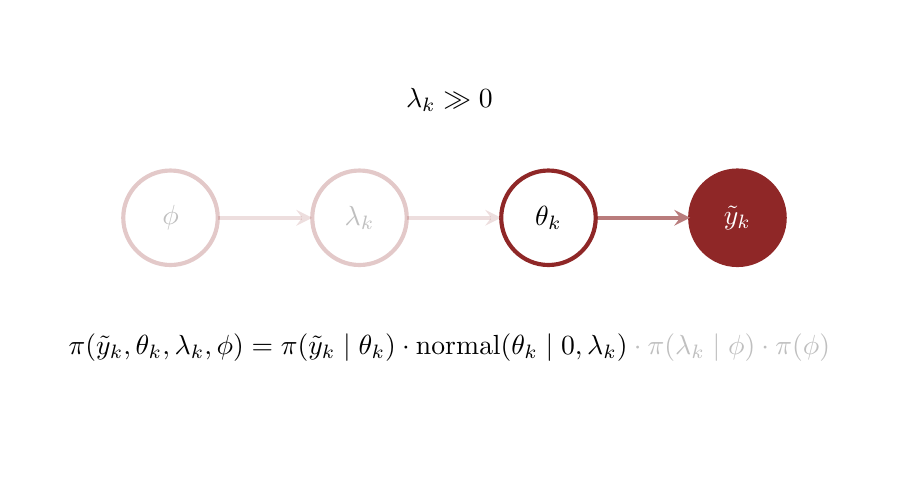
\begin{tikzpicture}[scale=0.3, thick]

\pgfmathsetmacro{\r}{2}

\pgfmathsetmacro{\dx}{0}
\pgfmathsetmacro{\dy}{0}

\draw[white] (-22 + \dx, -10 + \dy) rectangle (14 + \dx, 8 + \dy);

\node[align=center] at (-4 + \dx, 5 + \dy) 
{ $ \lambda_{k} \gg 0$ };

\node[align=left] at (-4 + \dx, -5.5 + \dy) 
{ $ \pi (\tilde{y}_{k}, \theta_{k}, \lambda_{k}, \phi) = \pi (\tilde{y}_{k} \mid \theta_{k} ) \cdot 
\text{normal}(\theta_{k} \mid 0, \lambda_{k}) \cdot \pi(\lambda_{k} \mid \phi) \cdot \pi(\phi)$ };

\fill[white, opacity=0.75] (3.5 + \dx, -6.5 + \dy) rectangle (13 + \dx, -4.5 + \dy);

\filldraw[fill=dark, draw=dark, dark, line width=1.5] (8 + \dx, 0 + \dy) circle (\r)
node[color=white] { $\tilde{y}_{k}$ };

\draw[->, >=stealth, color=mid, line width=1.5] 
  ({0 + \r + \dx}, {0 + \dy}) -- ({8 - \r + \dx}, {0 + \dy});

\filldraw[fill=white, draw=dark, line width=1.5] (0 + \dx, 0 + \dy) circle (\r)
node[color=black] { $\theta_{k}$ };

\draw[->, >=stealth, color=mid,  opacity=0.25, line width=1.5] 
  ({-8 + \r * cos(0) + \dx}, {0 - \r * sin(0) + \dy}) -- ({0 - \r * cos(0) + \dx}, {0 + \r * sin(0) + \dy});

\filldraw[fill=white, draw=dark,  opacity=0.25, line width=1.5] (-8 + \dx, 0 + \dy) circle (\r)
node[color=black] { $\lambda_{k}$ };

\draw[->, >=stealth, color=mid,  opacity=0.25, line width=1.5] 
  ({-16 + \r * cos(0) + \dx}, {0 - \r * sin(0) + \dy}) -- ({-8 - \r * cos(0) + \dx}, {0 + \r * sin(0) + \dy});

\filldraw[fill=white, draw=dark,  opacity=0.25, line width=1.5] (-16 + \dx, 0 + \dy) circle (\r)
node[color=black] { $\phi$ };

\end{tikzpicture}

\end{document}  